\chapter{Introduction}
\label{chap:introduction}

% Introduction should provide appropriate context and background for your research, such as the recent trend and importance of the technology development related to your thesis.

Non terrestrial network (NTN) has become a promising technique in next generation network. It provides network connectivity to area that traditional network platform cannot reach. For instance, forests, oceans, and deserts. Various platforms are used to provide network services in NTN, such as GEO, MEO, LEO satellites, UAVs, and drones. Among these platforms, LEO satellites are the most actively discussed. These satellites are located at altitude 500 to 2000 kilometers. The strongest advantage is that they provide global coverage, low latency, and high throughput compared to MEO or GEO satellites.

However, to acheive LEO satellite network service, there are some key challanges that need to be resolved. One of the challanges is the unavoidable frequent handover~\cite{38821}. The high speed of LEO satellite forces user equipments (UEs) on the ground to switch the serving satellites frequently, as shown in Figure~\ref{time to ho}. In such scenario, the signalling overhead led by handover signals and the handover interruption time are big issues. 3GPP has discussed some solutions to deal with these issues. By using quasi-earth-fixed cell and satellite switch with re-synchronization~\cite{38300}, the frequent handovers are avoided and the signalling overhead is reduced. For UEs that have already accessed to the network, they can receive the upcoming serving satellite information from the previous one. Also, with the help of the ephemeris data of satellies and the position information of UEs, the matching between satellites and UEs has been largely improved~\cite{38331}. Nontheless, for those UEs who have not access to the network, the random access procedure is the only way for them to get into the network. To establish the connection between satellites and UEs, satellites need to transmit synchronization signal block (SSB) to ground for UEs to capture. Once UEs have successfully receive SSBs, the random access procedure starts and the UEs are able to access to the satellite network. Typically in terrestrial network, ground stations send SSB to the serving area every 20 milliseconds. However, the traditional SSB specifications in LEO satellite communication system do not work because the power budget in LEO satellite is so tight that the power is not enough to send all the serving cells in such a short periodicity. Thus, in this thesis we will find out how to deal with this issue by adjust the SSB periodicity and transmitted power. 

\begin{figure}[h!]
    \centering
    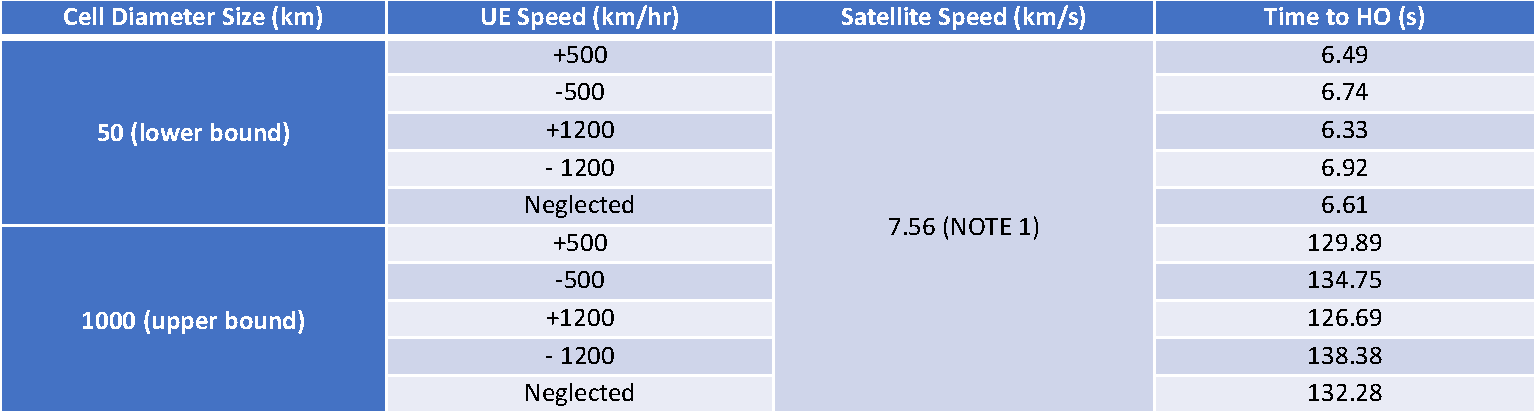
\includegraphics[width=1\textwidth]{figure/time to ho.pdf}
    \caption{Time to handover for min/max cell diameter and varying UE speed}
    \label{time to ho}
\end{figure}